\label{sec:data}
% Main characteristics of the data set: source, type of data
% Description of variables used for the	analysis and correspondence with the (ideal) magnitudes in the empirical specification
% Descriptive statistics of the	main variables in the analysis
Data for the analysis comes from a variety of sources. 
In general, we have three types of data: 
\begin{itemize}
    \item Airports. Data on airports. In the network setting, these correspond to nodes in the network.
    \item Flights/connections. These datasets contain information on flights or connections between airports. As will be described in detail below, we have access to a rich dataset on US flights, and a somewhat less extensive dataset on global connections. In the network setting, this information corresponds to links in the network.  
    \item Prices. Prices are generally harder to obtain in ready-to-use datasets. For this reason, we choose to scrape web-data on prices from \textit{Skyscanner}.
\end{itemize}

\subsection{Airport Data}
Data on airports comes from two overlapping sources. Firstly, we have a dataset from the 2009 Statistical Computing Data Expo\footnote{Available at \url{http://stat-computing.org/dataexpo/2009/}}. This dataset contains information 3376 US airports, and the unique IATA\footnote{International Air Transport Association} code, airport name, city, country and geographical location in WTS84 coordinates. This dataset contains 3.376 observations of individual airports. As will be described in \ref{subsec:Flight Data}, we only have information on flights/connections to and from a subset of these. A likely explanation is, that a number of these airports are not used for commercial air transport, but rather for e.g. training/sports purposes.\\
% Tjek at det reelt er WTS84 koordinater - det ser sådan ud. 
Secondly, we have a dataset on airports from OpenFlights\footnote{Available at: \url{https://openflights.org/data.html}}. This dataset contains the same information as the above, but further includes inter alia a unique 'OpenFlights identifier', ICAO code, and altitude. Furthermore, this dataset contains airports from all over the world. \\
We will primarily use the OpenFlights data, whenever the analysis has a global scope. This dataset contains information on 7543 individual airports. 

\subsection{Flight/Connection Data}
\label{subsec:Flight Data}
Flight data comes from the 2009 Statistical Computing Data Expo. Data is available for the period 1987-2008, and  includes information on almost 120 million commercial flights within the US. For each flight, we have a range of information, including the aircraft carrier, origin and destination (IATA coded), distance travelled, time in air date etc. For a single year (2007) there are 7.453.215 observations on a total of 29 variables. Flight data can be merged with airport data using the IATA codes on airports. \\
\\
We also have global connection data from OpenFlights. Connection data contains a single observation for a given route between airports, as opposed to observations for every single flight in the flights data. The dataset contains 67.663 directed connections between 3.321 airports. Note, that the connection data was last updated in 2014. Neither the connection data nor the flight data is thus up to date, and subsequent changes to the network will be a potential source of error in our analysis. 


%Data on airports and connections is available at: \href{https://openflights.org/data.html}{openflights.org/data.html}. See Figure \ref{fig:airports} below. The dataset includes an airport identifier (IATA code), location data (latitude and longitude), and various characteristics of the airport (country, city, altitude etc.).
%Furthermore, the dataset contains connections between airports (67,663 routes between 3,321 airports on 548 airlines). %Airports are identified using the IATA code.%we already mentioned this above
\medskip\\
%Data on prices are scraped from the internet. Various sites contain flight prices (Skyscanner, Momondo, Flightfinder, Expedia mv.). Our choice of site will be guided by practical concerns.
%\par
%Alternative data:  \url{http://stat-computing.org/dataexpo/2009/}
\begin{figure}[H]
  \centering
  \caption{Airports}
    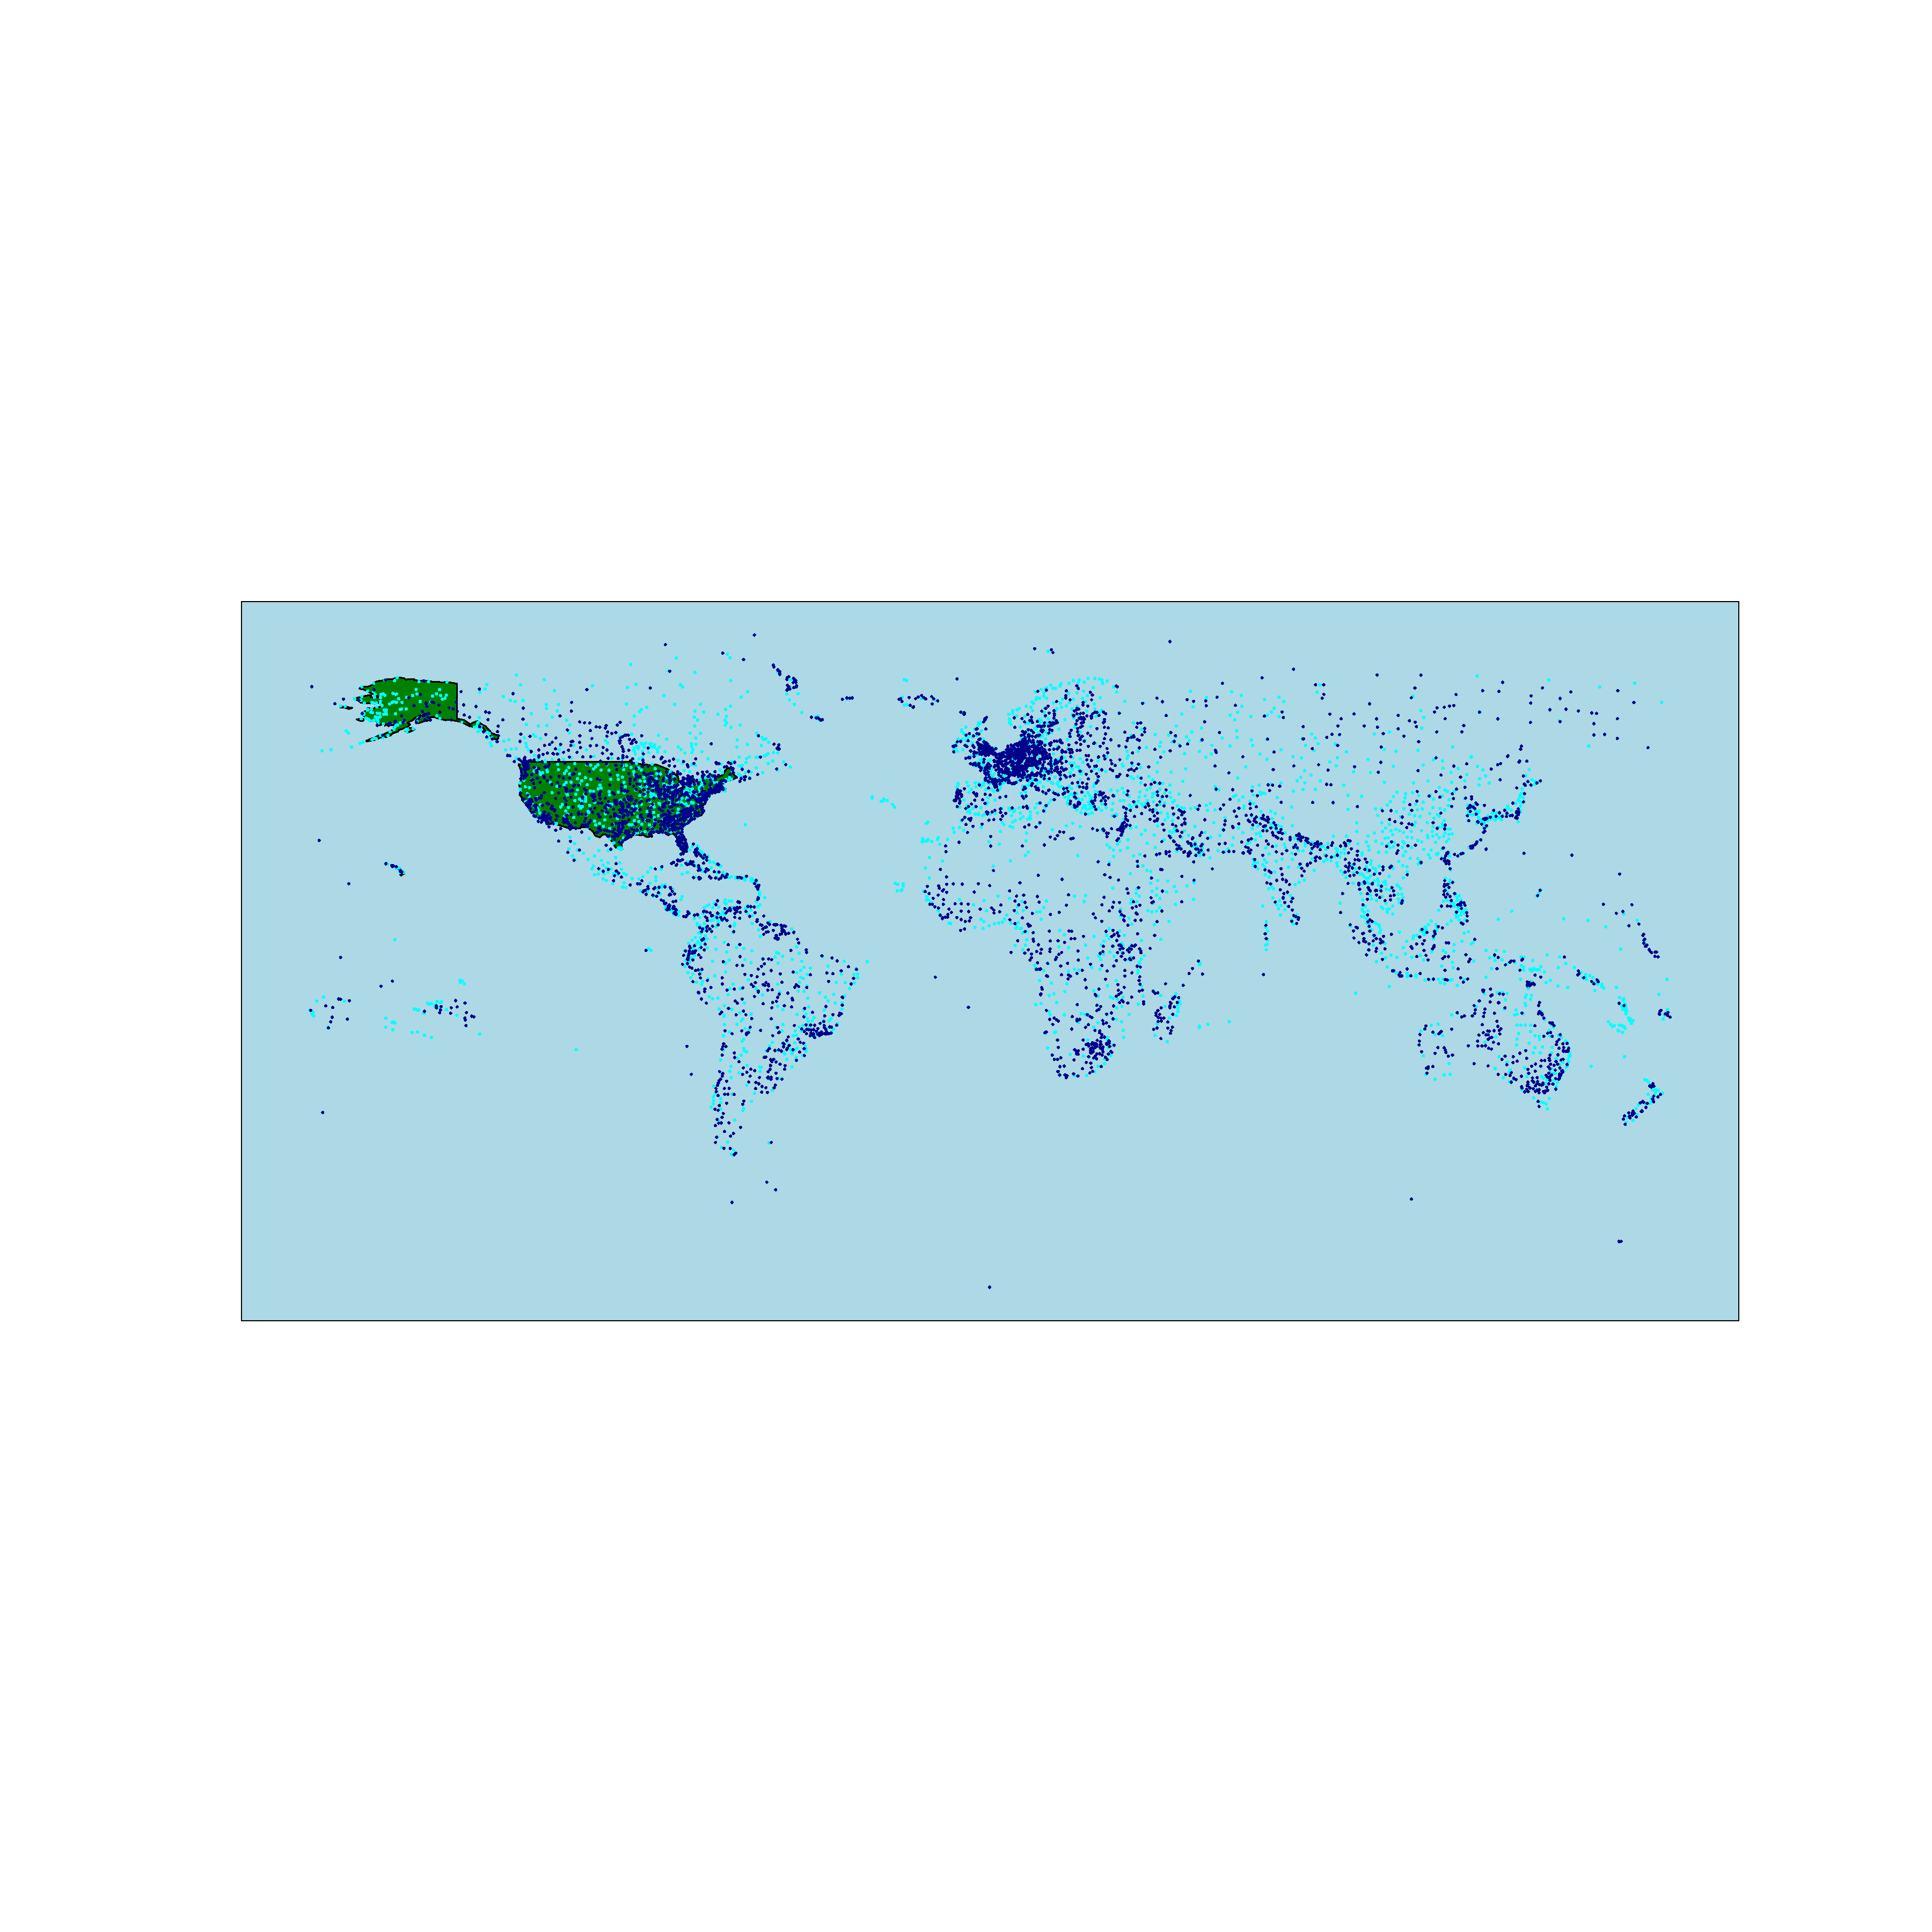
\includegraphics[width=1. \textwidth]{Exam/Airports_WorldMap}
  \label{fig:airports}
\end{figure}
